\documentclass[11pt]{article}
\usepackage[margin=1in]{geometry}                % See geometry.pdf to learn the layout options. There are lots.
\geometry{letterpaper}                   % ... or a4paper or a5paper or ... 
%\geometry{landscape}                % Activate for for rotated page geometry
%\usepackage[parfill]{parskip}    % Activate to begin paragraphs with an empty line rather than an indent
\usepackage{color}
\definecolor{myblue}{rgb}{0.0, 0.0, 0.85}
\usepackage[breaklinks=true, colorlinks=true, linkcolor=red, urlcolor=myblue, citecolor=black]{hyperref}
\urlstyle{rm}
\usepackage{mathptmx}
\usepackage{graphicx}
\usepackage{amssymb}
\usepackage{epstopdf}
\usepackage{sidecap}
\usepackage{authblk}
\usepackage{booktabs}
\usepackage[font=small,labelfont=bf]{caption}
\usepackage{enumitem}
\usepackage{wrapfig}
\DeclareGraphicsRule{.tif}{png}{.png}{`convert #1 `dirname #1`/`basename #1 .tif`.png}
\pagestyle{plain}

\def\bfr{\bf\color{red}}
\def\bfp{\color{magenta}}
\def\geohub{{\tt geohub}}
\def\resp{respectively}
\def\selah{SELAH}

\begin{document}
%\maketitle

\begin{center}
	\Large\bf Unsheltered Homelessness in Hollywood Is Down from January 2020 Levels\\
	\vspace{1ex}
	{\normalsize\rm Louis Abramson, PhD, and Brian Kohan 
	for the \href{http://www.hollywood4wrd.live}{\it Hollywood4WRD Coalition} \\ \today 
	{\bfr \texttt{ -- NOT FOR DISTRIBUTION}}}
\end{center}

\noindent {\bf Summary:} A February 25, 2021 census of Hollywood and East Hollywood suggests that 
unsheltered homelessness has fallen in those communities by $11\%$ and $15\%$, \resp, compared to 
the 2020 LAHSA Point-In-Time (PIT) count. A 30\% drop in individuals seen on the street drives this 
change (Figure \ref{fig:rawCounts}), reducing the number of identified persons and dwellings in 
about a third of census tracts. Unsheltered living is thus likely to have declined quantitatively even if the 
average number of people living, e.g., in tents is updated. {\bfp Simultaneously, however, 13\% of tracts
saw at least a doubling in street dwellings. Combined with the salient side-effects of COVID-related 
reductions in health, hygiene, and social support services, this trend may contribute to accurate 
perceptions that the state of homelessness has worsened over the past year, albeit at reduced scale.} 
Coordinated Entry System data will reveal whether homelessness has declined in toto or 
if government initiatives reduced only the portion of people living unsheltered in Greater Hollywood.
%This trend holds in tracts assessed by professionals or volunteers and is larger 
%than counting errors can account for.
% less than a 93\% chance that 
%with at least one preliminary survey suggesting such updates may be modest
%the number of unsheltered people has fallen by at least some amount. %\pm9\% %\pm12\%
%(1/23)
%assuming no changes in average dwelling occupancies, 
%Only seven tracts saw significant increases in raw counts, with makeshift dwellings the only category to increase in both CoCs. 
%All data are available to support future analyses incorporating such information.

\begin{figure*}[h]
	\centering
	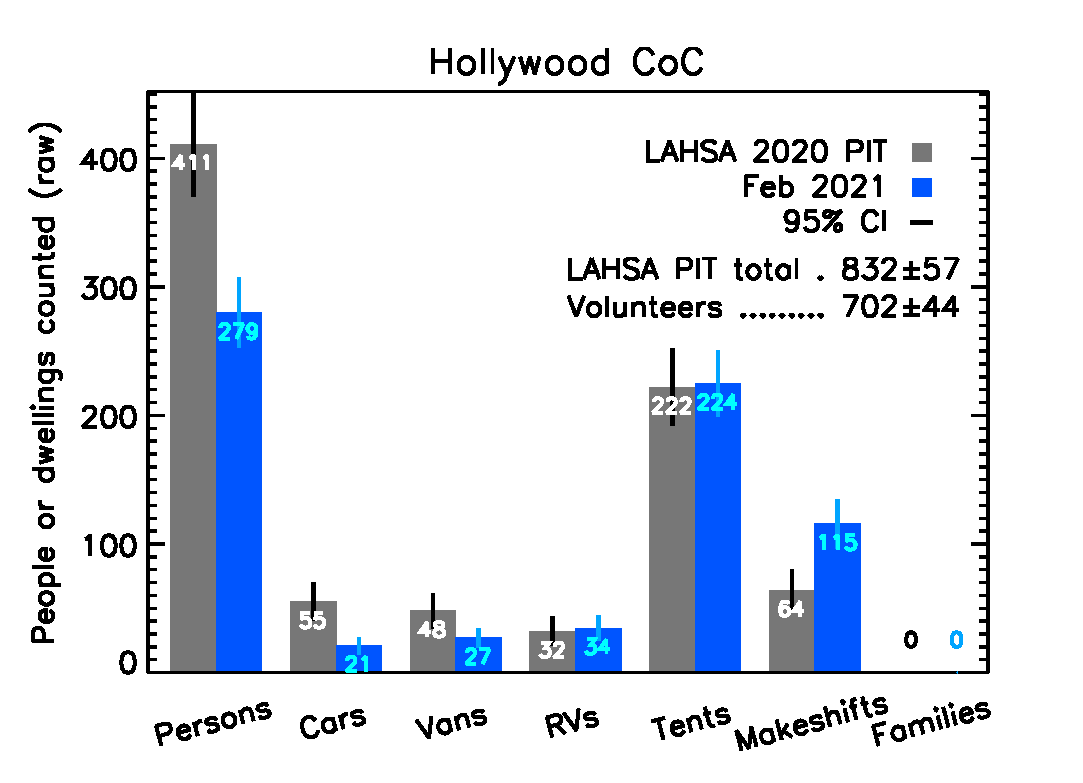
\includegraphics[width = 0.47\textwidth, trim = 1cm 0cm 0cm 0cm]{Hwood2021Bars}
	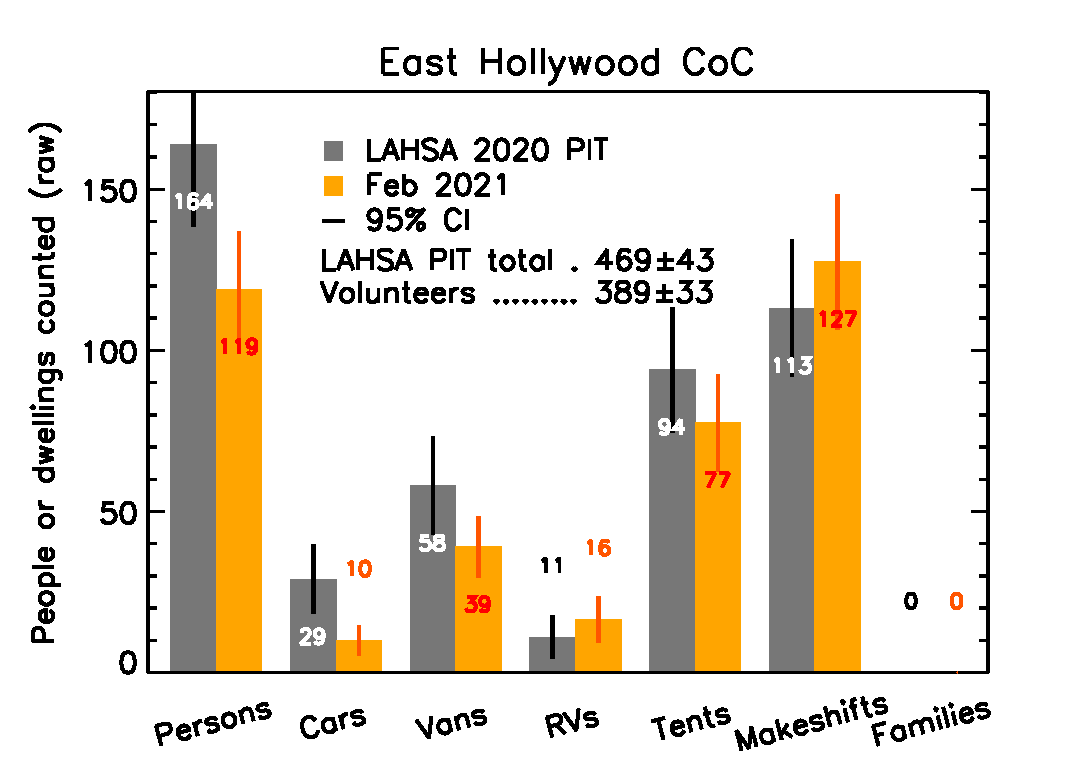
\includegraphics[width = 0.47\textwidth, trim = 0cm 0cm 1cm 0cm]{Eho2021Bars}
	\caption{Raw tallies of unsheltered persons and dwellings in Hollywood and East Hollywood
			(left/right) from the 2020 and 2021 PIT counts (grey/colors). Persons, cars, 
			and vans fell in both communities while RVs and tents stayed statistically flat. 
			Makeshift structures are the only category to show a potential common increase. 
			Overall, we identified 208 fewer people and dwellings compared to 2020,
			with similar 16\% decreases assessed by almost entirely independent teams
			in both communities. ``Persons'' are TAY+Adults.}
	\label{fig:rawCounts}
\end{figure*}

\begin{table*}[h!]
\caption{Greater Hollywood 2021 PIT Unsheltered Data and Population Estimates}
\resizebox{\linewidth}{!}{%
\begin{tabular}{lcccccccccc}
\toprule
 & Adult & TAY & Car & Van & RV & Tent & Makeshift & {\bf 2021 Total} & {\bf 2020 Total} & {\bf Difference} \\ \cmidrule{1-11}
{\bf Hollywood} \\ %\cmidrule{1-1}
Counts & 277 & 2 & 21 & 27 & 34 & 224 & 115 & {\bf 702} & {\bf 831} & $\bf -15\%$ \\
Inhabitants & 277 (27) & 2 (5) & 32 (11) & 49 (13) & 50 (14) & 332 (29) & 195 (24) & {\bf 937 (93)} & {\bf 1058} & $\bf -11\%\,(9\%)$\\% (76)
Category share & 30\% (3\%) & 0\% (0\%) & 3\% (1\%) & 5\% (1\%) & 5\% (1\%) & 35\% (3\%) & 21\% (3\%) & -- & -- & -- \\ \cmidrule{1-11}
{\bf East Hollywood} \\ %\cmidrule{1-1}
Counts & 114 & 4 & 10 & 39 & 16 & 77 & 127 & {\bf 389} & {\bf 469} & $\bf -17\%$ \\
Inhabitants & 114 (19) & 4 (4) & 15 (8) & 70 (15) & 24 (9) & 115 (19) & 216 (23) & {\bf 557 (83)} & {\bf 656} & $\bf -15\%\,(12\%)$\\% (60)
Category share & 20\% (3\%) & 1\% (1\%) & 3\% (1\%) & 13\% (3\%) & 4\% (2\%) & 20\% (3\%) & 39\% (4\%) & -- & -- &--
\\ \bottomrule
\end{tabular}
}
\caption*{Parentheses denote 90\% uncertainties. Uncertainties larger than estimates 
imply that only upper limits are available. No unaccompanied minors or families were observed.}
\label{tbl:summary}% (binomial in the case of the categories)
\end{table*}

\begin{figure*}[t]
	\centering
%	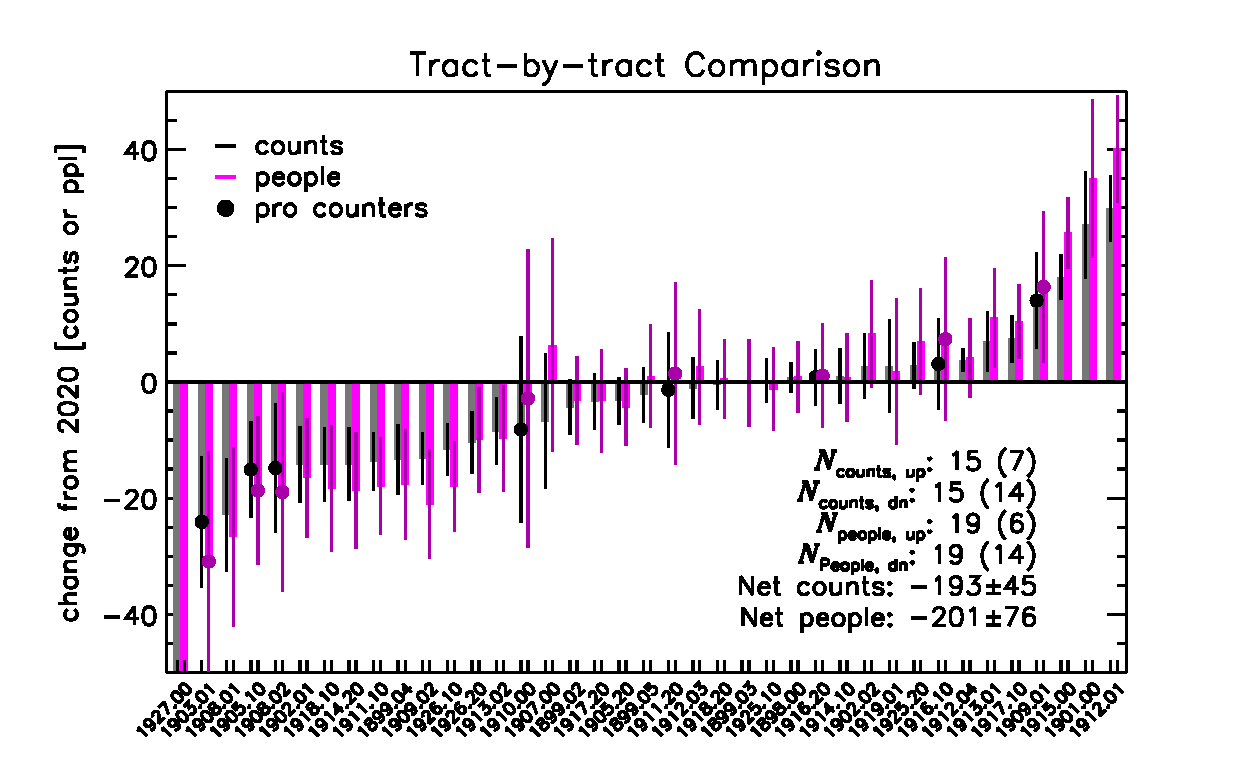
\includegraphics[width = 0.8\textwidth, trim = 0cm 0cm 0cm 0cm]{tractsYrYr}
	\includegraphics[width = 0.8\textwidth, trim = 0cm 0.25cm 0cm 0.25cm]{countMap}
	\caption{The Greater Hollywood PIT survey area with census tracts colored by inferred 
			changes in total unsheltered population from 2020 (red$+$, blue$-$).
			Hollywood (21 tracts) spans Crescent Heights/Franklin to 
			Western/Melrose; East Hollywood (18 tracts) spans Hollywood/Western 
			to Hoover/Beverly. East Hollywood saw to the largest tract-level changes,
			with 1912.01 (NE box, volunteer-tallied) rising by 40 people and 1927.00 
			(SE box, pro-tallied) falling by over 120 people. Subsequent cross-checks 
			support both tracts' PIT counts.}
	\label{fig:tcomp}
\end{figure*}

%\begin{figure*}[h!]
%	\centering
%	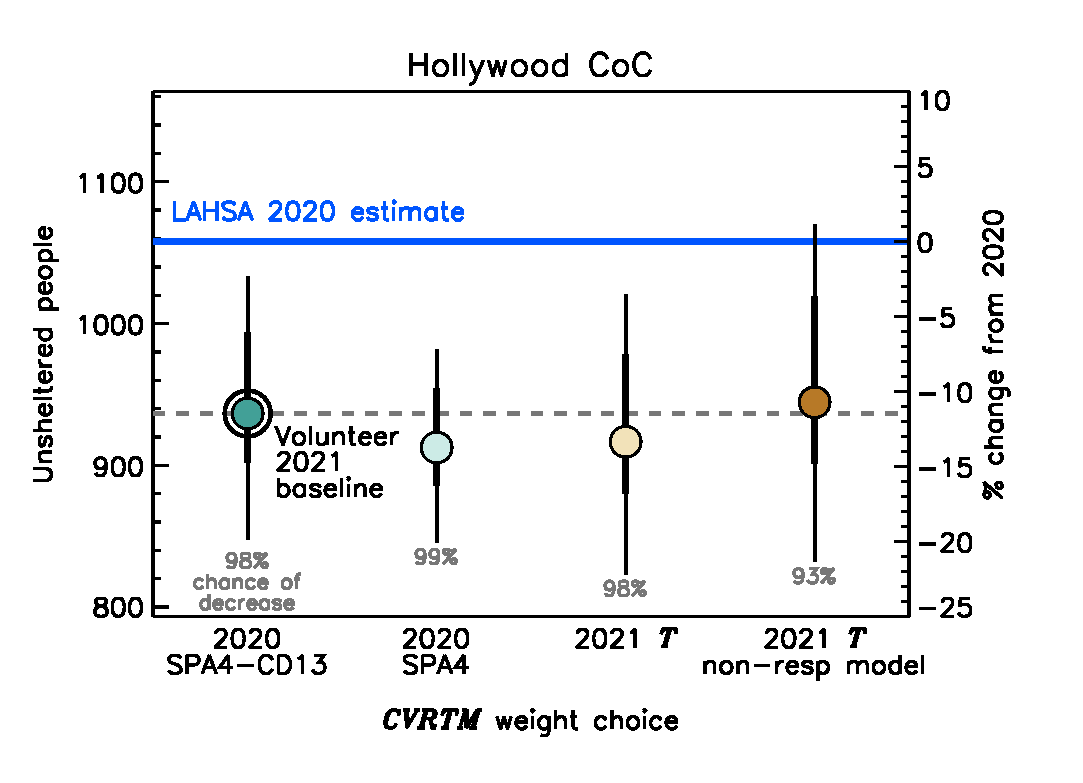
\includegraphics[width = 0.48\textwidth, trim = 0cm 0.5cm 0cm 0cm]{hwoodFinal}
%	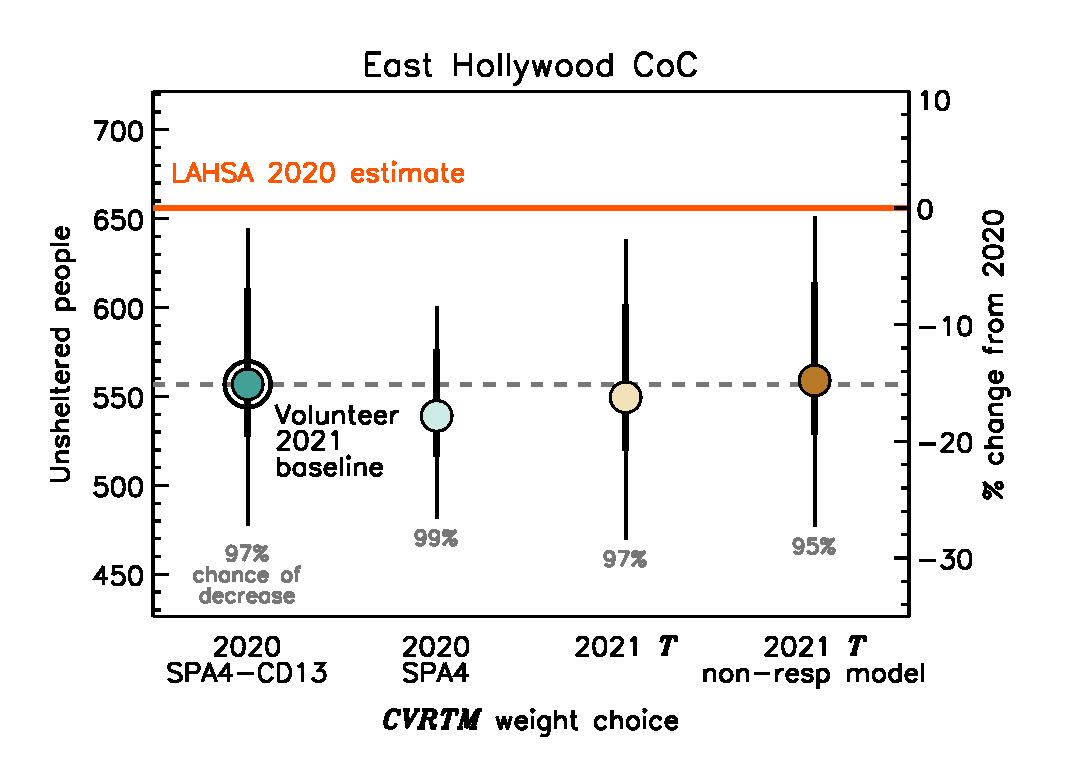
\includegraphics[width = 0.48\textwidth, trim = 0cm 0.5cm 0cm 0cm]{ehoFinal}	
%	\caption{Unsheltered populations in Hollywood (left) and East Hollywood (right) 
%			as functions of CVRTM weights. The baseline estimate uses the same weights as the 
%			2020 LAHSA Community Summaries. Using SPA4 weights or replacing the tent 
%			weight, $T$, with results from a survey conducted in Hollywood yields consistent
%			results. All imply at least a 93\% chance that unsheltered homelessness has fallen
%			by some amount, with likely declines of $12\%\pm9\%$ and $15\%\pm12\%$
%			in Hollywood and East Hollywood, \resp.}
%	\label{fig:wtComp}
%\end{figure*}

\pagebreak

\noindent {\bf Context:} Government, nonprofit, and volunteer organizations in Hollywood---{\it \href{https://thecenterinhollywood.org}
{The Center at Blessed Sacrament}, \href{https://chnc.org}{The Central Hollywood Neighborhood Council}, 
\href{https://www.covenanthouse.org/spring-meal-match?sourceid=2483460&origin=DHQEI2109EZI0N&utm_source=2103marchmealmatchweb&utm_medium=cpc&utm_campaign=FY21MarchMealMatch&utm_content=bsd2103marchmealmatchweb&gclid=CjwKCAiAp4KCBhB6EiwAxRxbpJA2yM7lM2tyAqjVALZgBGvjnhobCJJ0XmuELFDXzM5xxZ0BqyX1ChoCLi0QAvD_BwE}{Covenant House}, 
Hang Out Do Good, \href{https://hollywood4wrd.live}{Hollywood4WRD}, 
 \href{https://www.myfriendsplace.org/}{My Friend's Place}}, and various resident organizers---conducted 
a PIT enumeration of people experiencing unsheltered homelessness to compensate for 
the \href{https://laist.com/latest/post/20201209/LAHSA-cancels-2021-homeless-count-los-angeles-covid-19}
{cancellation} of the official 2021 Count. All 39 US Census tracts in the LAHSA-recognized Hollywood 
and East Hollywood communities were surveyed on 25 February (Figure \ref{fig:tcomp}). Nine tracts 
were counted by professional outreach teams during the %---comprising $\sim$43\% of identified individuals and dwellings---
day. The remainder were surveyed by car-based volunteer teams beginning at 7:00 PM.

Each volunteer team was assigned two tracts in one of the communities. Given high turnout, each tract was 
surveyed by at least two teams, increasing the accuracy of the count. Tracts 
surveyed by professionals were counted only once. No volunteer teams and only one professional team counted 
tracts in both communities, making the two datasets almost entirely independent.
%and enabling better error estimates

Year-on-year trends are consistent across communities and between volunteer- and professional-counted tracts.
Six tracts saw significant population increases and 14 saw declines. The tracts with the largest increase (1912.01;
Barnsdall Park) and decrease (1927.00; US Rte.\ 101) are both in East Hollywood.\\
%; volunteer-counted; professional-counted

\noindent {\bf Results and uncertainties:} The population inferences in Table \ref{tbl:summary} %and Figure \ref{fig:wtComp} 
reflect 10,000 Monte Carlo resamplings of the survey data with 
counts perturbed randomly by their uncertainties. Counts for cars, vans, RVs, tents, and 
makeshift dwellings (CVRTM) were additionally boosted by the relevant mean occupancy weights 
perturbed by their own uncertainties. The baseline case adopts the 2020 
%quoted in Table \ref{tbl:summary} and shown in teal in Figure \ref{fig:wtComp}
\href{https://www.lahsa.org/documents?id=4635-usc-2018-2020-multipliers-and-estimates-overview}
{SPA4/CD13 CVRTM weights} underpinning the latest official Hollywood and East Hollywood 
\href{https://www.lahsa.org/documents?id=4686-2020-greater-los-angeles-city-community-homelessness-report-service-planning-area-4.pdf}
{Community Summaries}, from which we also draw 2020's person and CVRTM raw tallies. Those inferences yield 
$936\pm92$ and $556\pm83$ people experiencing unsheltered homelessness, \resp\ (90\% CI). Modifying the weights
to their 2020 \href{https://www.lahsa.org/documents?id=4693-2020-greater-los-angeles-homeless-count-cvrtm-conversion-factors}
{SPA4-wide} values or using data from in-person surveys of tent-dwellers in Hollywood has no
significant effect.\footnote{Respectively, those inferences suggest $912\pm68$ and $944\pm118$ people
in Hollywood, and $539\pm59$ and $559\pm87$ in East Hollywood, consistent with baseline results.} 
All estimates suggest at least a 93\% chance of a decline compared to the 2020 PIT count.
 % (Figure \ref{fig:wtComp})

Nevertheless, the CVRTM weights are systematic uncertainties. If, on average, more people today live in each tent 
or makeshift structure compared to last year, then some of our inferred population decline would be artificial. 
However, the drop in unweighted counts is such that the occupancy increases needed to erase our estimated changes are
substantial. All else being equal, the {\it average} tent would need to shelter 2 people in Hollywood and 2.8 people in 
East Hollywood vs.\ 1.5 people in 2020. The average makeshift structure would need to shelter 2.7 and 2.5 people, 
\resp, vs.\ 1.7 people a year ago. Such 30\%--90\% increases in {\it mean} occupancies seem unlikely given 
known COVID-related tent distribution efforts pushing in the opposite direction, and a 28 Feb.\ tent survey 
yielding a weight consistent with 2020's value.\footnote{The $T$ and $M$ weights are the largest 
potential error sources in this analysis due to the high proportion of people living in tents and makeshift structures. 
While the full 2021 PIT area has not been assessed, \selah\ outreach teams surveyed 47 tents (38 responses) in 
Hollywood on 28 Feb., yielding a mean occupancy of $T=1.39\pm0.14$ people per tent ($T=1.50\pm0.22$ when 
non-responses are modeled). Although $M$ was not estimated, that $T$ value is consistent with the official 2020 
weight of $T=1.48\pm0.11$. We encourage more robust efforts to update the CVRTM weights.} 

{\bfr SAFE PARKING NUMBERS}

Multiple cross-checks suggest that the raw counts from our 2021 PIT enumeration are accurate:
\begin{enumerate}
%	\setlength{\itemsep}{-1ex}
	\item Comparisons of the count's 37 duplicate tract measurements suggest per-tract and per-category
		counting uncertainties are consistent with the random errors built into the analysis.
%		\begin{itemize}
%			\item Tract 1901.00---the only outlier in the above comparisons---was independently recounted 
%				14 hours after the PIT count with results consistent with the average of the volunteer teams' 
%				results.
%			\item Tract 1912.01---largest increase---was independently recounted on 27 Feb.\ circa 
%				12:00 PM with results similarly consistent with the PIT teams' assessments.
%			\item Tract 1927.00---largest decrease---was independently recounted on 4 March at 
%				8:30 AM with results lower than the PIT's assessment. This especially dense tract was originally 
%				surveyed on foot by outreach professionals, however, with the recount was performed by a car-based
%				volunteer. The cross-check therefore suggests only that the PIT data are not biased in ways that
%				would induce an artificial year-on-dear decline.				
%		\end{itemize}
	\item External data from \href{https://hollywoodpartnership.com/}{\it The Hollywood Partnership} 
		from 19 Feb.\ are consistent with both our PIT count in a common tract (1902.02) and an independent 
		recount of that entire geography performed 28 Feb.% also show a decline from past values and 
	\item Tracts counted by volunteer and professional teams show consistent trends.
	\item Counts in Hollywood and East Hollywood show consistent trends.% (reduced individuals, flat
%		or marginally higher dwelling counts).
%	\item Tracts monitored by \selah\ since May 2020 show similar declines to that implied by our data. 
%		One of these tracts is 1912.01 in East Hollywood, whose 27 Feb.\ \selah\ estimate  agrees with our 
%		PIT value.% in unsheltered homelessness.
	\item A 27 Feb.\ recount of tract 1912.01 in East Hollywood conducted as as part of a
		\href{https://selahnch.org}{\selah} monitoring campaign agrees with our PIT value.% in unsheltered homelessness.
\end{enumerate}

%		   P	C     V	    R	 T     M
%1901.00 -- 50    8    5.5   1     6      4 -- 2021, raw
%1901.00 -- 36    4     6     0     8      2 -- 26 Feb ABRAMSON 9.00 AM
%
%1927.00 -- 48    1      5     0    53    70 -- 2020, raw
%1927.00 -- 20    0     0     7     6     54 -- 2021, raw
%1927.00 -- 15     0     9     5    14    21 -- 4 Mar 2021 ABRAMSON 8.45 AM
%
%1912.01 --  18.5  0.5  3.5  1.5  5.5  12 -- 2021, raw
%1912.01 --  21     0      4     1     8      6  -- 27 Feb ABRAMSON 12.15 PM
%
%1902.02 -- 9      --     --     --     8   5.5 -- 2021, raw
%1902.02 -- 9      --     --     --    17    --  -- BID 2/19

% 1907.00 is also interesting in that total population stayed nearly the same but identified
% individuals and dwellings basically swapped: IND 73->38; CVRTM 31->70. This has a big impact
% on people's perceptions, and it's in a very high-traffic part of the community.

%The pro/vol trends are consistent everywhere except tract 1927.00, 
%			where pro counts dropped significantly more for both individuals and dwellings (esp.\ 
%			tents). 1927.00 comprises 22\% of total counts in East Hollywood. Unsheltered 
%			homelessness in that CoC was flat or rose slightly outside of that tract.}
%{\bfr 1927.00 is the tract with the PATH Madison PSH. Phase II opened in Jan 2020---leasing began May 
%2020---and is 120 units, some of which were filled from nearby folks but I dunno how many. LEA recounted 
%this tract 4 March at $\sim$9:00 AM and found 94 total population vs.\ pro's 129. Only place where
%LEA counted more objects was vans. Adding that to the pro total adds 16 people (9 vans).

All of the above suggests that our results are both quantitatively and qualitatively reliable.\\

\noindent {\bf Comments:} The decline we find is largely driven by a $\sim$30\% drop in observed 
unsheltered individuals in both Hollywood and East Hollywood. This reduction may be partially attributable to 
government initiatives aimed at moving people indoors (Project Roomkey) and staunching inflow into homelessness 
(eviction moratoria). Examining Project Roomkey, \href{https://www.lahsa.org/documents?id=4672-2020-homeless-count-council-district-13}
{CD13's} share of \href{https://www.lahsa.org/documents?id=4585-2020-greater-los-angeles-homeless-count-los-angeles-continuum-of-care-coc-}{LA County's total unsheltered senior population} (6.5\%) implies that perhaps 100 of its 
\href{https://projectroomkeytracker.com/}{1608 occupied rooms} were filled with Greater Hollywood 
residents on the night of the PIT count---enough to account for about half the inferred change. 
The opening of at least one {\it A Bridge Home} site in Los Feliz {\bfr Five ABH's cover Greater Hollywood,
three have catchment areas covering 1927.00. Their net addition is 33 beds, total, but 89 in that tract (whose
net gain is eroded by losses of preexisting beds from Schrader and Garnder in the west).}---whose 
catchment area includes Hollywood---may 
also have contributed, as might the opening of 120 permanent supportive housing units by PATH in May 2020 
in tract 1927.00. While all of the latter rooms did not go to local unhoused residents, some may have, thus 
helping drive that tract's large observed decrease. 

Data from the Coordinated Entry System should constrain the above possibilities, revealing whether homelessness 
writ large has fallen since 2020, or just the unsheltered share in Greater Hollywood.

If the numbers have fallen, however, conditions for those left on the street have also degraded due to COVID-related 
closures of restaurants and other facilities proving basic support to unhoused people (food, hygiene). Reduced sanitation 
activity and access to mental health and drug treatment centers {\bfr (VERIFY, add overdose data)} have only exacerbated those challenges. 
Hence, while these data may support the efficacy of programs designed to reduce street homelessness, they do not suggest 
that the state of homelessness in Greater Hollywood has improved. In the fight to rebuild lives---as well as build homes---that fact 
cannot be forgotten.

{\bfr VISUAL DISPLAY VS NUMBERS -- SEE PEOPLE WHO'VE MOVED TO VALLEY RETURNING 
TO HOLLYWOOD FOR SERVICES DURING THE DAY.}

DPSS closed; phone system with long waits req'd to replace EBT. If you don't have a phone your stuck.

Libraries are closed, and therefore {\it The Source} service connection events. Daytime charity resources and some parks are 
closed, resulting in more exposure to the weather and less food.

Med-Cal not accessible via DPSS. Enrolling in health insurance requires similar phone calls and that a state ID be uploaded 
(previously not required). Lacking insurance affects likelihood and length of admission to hospital. Discharges requiring skilled 
or recuperative care placements are even more difficult.

DMV is by appointment only and appointments are made online.

DMH clinic services done via telehealth, leaving homeless clients hanging. One FSP has abandoned all field work due to COVID. 
Clients in crisis needing evaluations redirected to hospitals.

Hospitals, IMD's step down facilities and SNF's do not allow visitors, limiting the ability of case managers to negotiate 
with clients and social workers to ensure successful discharges. Consent forms for sharing info cannot be signed by patients 
due to lack of access.

Homeless people have gotten sicker while hospitals and LAFD have become overburdened dealing with COVID fallout, 
resulting in less access to emergency care.

%HOLLYWOOD -- Zero delta requires CVRTM mean occupancies of:\\
% - 5.00 ppl/car (from 1.51)\\
% - 5.00 ppl/van (from 1.77)\\
% - 4.95 ppl/RV (from 1.42)\\
% - 2.03 ppl/tent (from 1.48)\\
% - 2.73 ppl/mkshft (from 1.68)\\
%
%EAST HOLLYWOOD -- Zero delta requires CVRTM mean occupancies of:\\
% - 5.00 ppl/car (from 1.51)\\
% - 4.33 ppl/van (from 1.77)\\
% - 5.00 ppl/RV (from 1.42)\\
% - 2.78 ppl/tent (from 1.48)\\
% - 2.45 ppl/mkshft (from 1.68)


% ------ SUMMARY for HWOOD ------ 
%
%Total People (90%CI) .   936+/-92
%Fraction vs. last yr .   0.89+/-0.09
%Total counts..........   702
% > Adults    : 277 (39%), 277, (29%)
% > TAY       :   2 ( 0%),   2, ( 0%)
% > Minors    :   0 ( 0%),   0, ( 0%)
% > Cars      :  21 ( 2%),  31, ( 3%)
% > Vans      :  27 ( 3%),  47, ( 5%)
% > RVs       :  34 ( 4%),  49, ( 5%)
% > Tents     : 224 (31%), 330, (35%)
% > Makeshifts: 115 (16%), 193, (20%)
% > Families  :   0 ( 0%),   0, ( 0%)
%% Compiled module: MINMAX.
%Min/max ppl/tract ..... 0, 169
%Min/max counts/tract .. 0, 123
%
% ------ SUMMARY for EHO ------ 
%
%Total People (90%CI) .   556+/-83
%Fraction vs. last yr .   0.85+/-0.13
%Total counts..........   389
% > Adults    : 114 (29%), 114, (20%)
% > TAY       :   4 ( 1%),   4, ( 0%)
% > Minors    :   0 ( 0%),   0, ( 0%)
% > Cars      :  10 ( 2%),  14, ( 2%)
% > Vans      :  39 (10%),  68, (12%)
% > RVs       :  16 ( 4%),  23, ( 4%)
% > Tents     :  77 (19%), 114, (20%)
% > Makeshifts: 127 (32%), 214, (38%)
% > Families  :   0 ( 0%),   0, ( 0%)
%Min/max ppl/tract ..... 6, 129
%Min/max counts/tract .. 5, 87


%\begin{wrapfigure}{r}{0.5\linewidth}
%	\centering
%	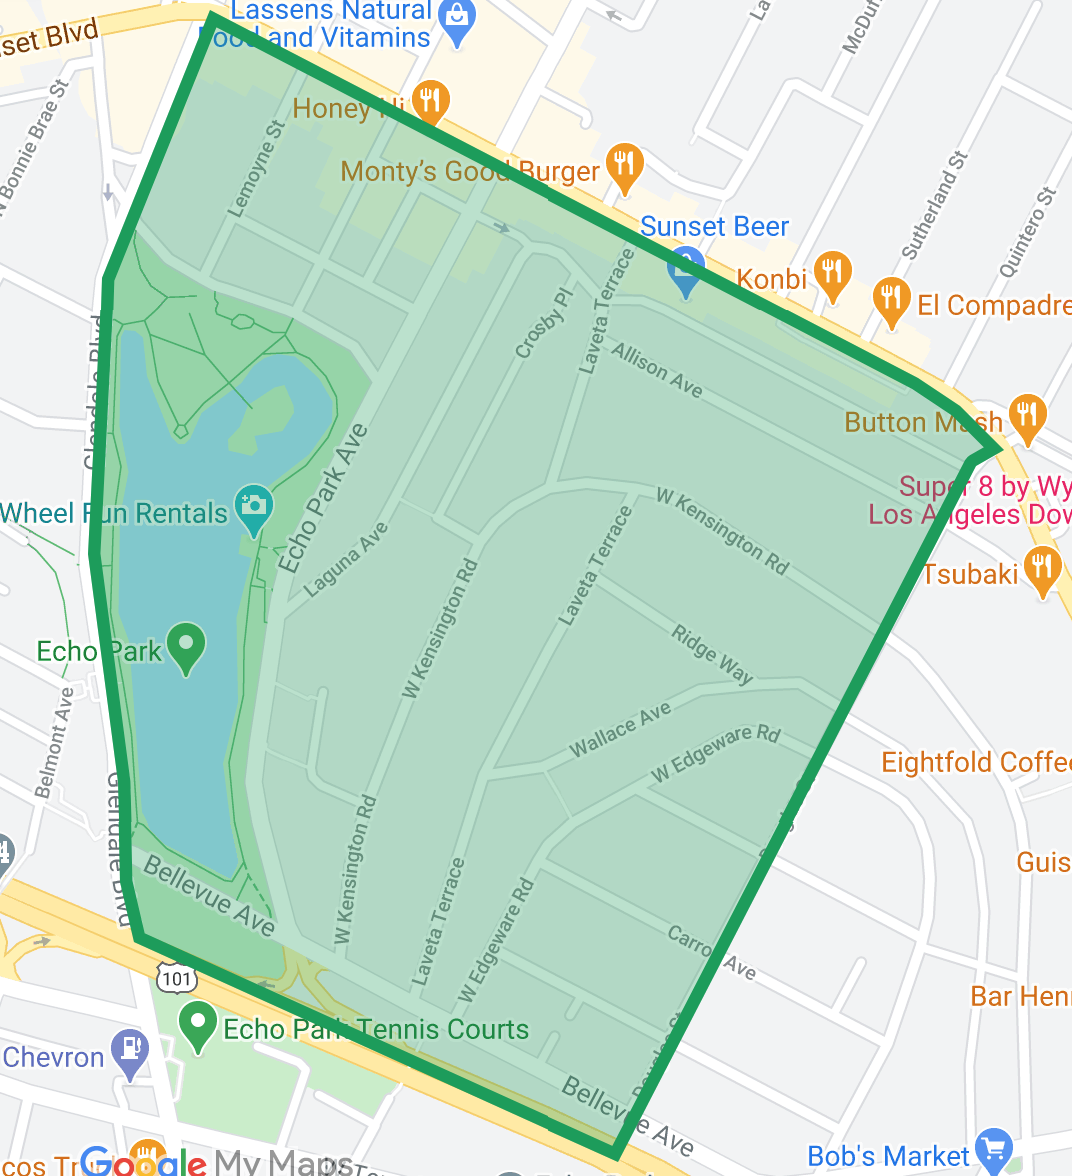
\includegraphics[width=\linewidth]{t1975}
%	\caption{US Census tract 1975.00.}
%	\label{fig:tract}
%\end{wrapfigure}
%\noindent {\bf Context:} \selah\ volunteers performed two recounts of US Census tract 1975.00 
%on 2 August and 18 October 2020 (Figure \ref{fig:tract}). This tract contains Echo Park Lake and various 
%CalTrans lands. The results of both surveys were statistically identical except for the estimate of vans, 
%which rose from $14\pm3$ to $25\pm5$ between counts. Our final individual/dwelling statistics 
%(Table \ref{tbl:rawData}) and total population estimates (Figure \ref{fig:results}) reflect the average 
%of those assessments.\\

%{\bfr KANAGI: ``we've seen a visual drop; dunno where they went but...'' On 2/18 they found 136 
%total tents in the BID vs our 127 (I haven't vetted the rest of the lines; that's just 12\# hot so w/e). (Also 99
%ppl compared to our 89, and 7 vehicles to our 10 and we weren't tracking those as hard as tents.) 
%On the 5th, they counted 163. That's a 17\% decline in 2 weeks, a little more that what we've seen year on year.
%Suggests maybe something happened in early Feb.? -- 3/2 @ 9:55 AM. The tent+mkshft count in 1902.02 is also 
%right on..}

%Only seven tracts saw significant increases in raw counts, with makeshift dwellings the only category to increase in both CoCs. 

%
%
%Cars and vans are hard to count, but there's no evidence of a bias. I repeated the most deviant tract the next day, 
%and another tract the day after that. In the latter case, both of my estimates were 0.5 units off the mean, in the 
%former, vans were at that level and I counted fewer cars. Brian and I also recovered a consistent amount of vehicles 
%with the BID (10 vs. their 6 separated by 20+ days). The rest of the tracts show a mean inter-counter bias of 0.6 
%cars (0.4 std.~err) and 1.24 ($0.76\sigma$) vans across all tracts, which should be accounted for in the MC.


% Pro teams counted areas comprising $\sim$43\% of the total raw counts. Three out of these 4 tracts 
% were counted by Covenant House teams, but 1927.00 has the largest drop of any tract and is Elyse 
% from The Center. That tract is basically responsible for the entire decline in East Hollywood, and most 
% of that is in reduced tents, so we should 	talk to these teams.


\end{document}  